% WSCG sample document 
%
% based on Gabriel Zachmann's sample
% http://zach.in.tu-clausthal.de/latex/
%
% modified Apr 2012 to match WSCG Word template
%
\documentclass[twoside,twocolumn,10pt]{article}
%\documentclass[twoside,twocolumn,draft]{article}

%  for debugging
%\tracingall%\tracingonline=0
%\tracingparagraphs
%\tracingpages

\usepackage{biblatex}
\usepackage[utf8]{inputenc}
\usepackage{amsmath}
\addbibresource{references.bib}

\usepackage{subfig}




%%%%%%%%%%%%%%%%%%%%%%%%%%%%%%%%%%%%%%%%%%%%%%%%%%%%%%%%%%%%%%%%%%%%%%%%%%%%%
%                             Packages

\usepackage{wscg}           % includes a number of other packages (e.g., myalgorithm)
\RequirePackage{ifpdf}
\ifpdf
 \RequirePackage[pdftex]{graphicx}
 \RequirePackage[pdftex]{color}
 
\else
 \RequirePackage[dvips,draft]{graphicx}
 \RequirePackage[dvips]{color}
\fi
%\usepackage[german,english]{babel}     % default = english
%\usepackage{mypicture}      % loads graphicx.sty, color.sty, eepic.sty
%\usepackage{array}          % better tabular's & arrays, plus math tabular's
%\usepackage{tabularx}      % for selfadjusting p-columns
%\setlength{\extrarowheight}{1ex}   % additional space between rows
%\usepackage{booktabs}      % typographically much better
%\usepackage{mdwlist}        % for compacted lists, and more versatile lists
%\usepackage[intlimits]{amsmath} % more math stuff, see texdoc amsldoc
%\usepackage{mymath}         % own commands, loads amssymb & array.sty
%\usepackage{hyphenat}      % hyphenatable -, /, etc.
%\usepackage{theorem}
%\usepackage[sort&compress]{natbib}% better \cite commands, more flexible
%\usepackage[sort&compress,super]{natbib} % better \cite commands, more flexible
%\newcommand{\citenumfont}[1]{\textit{#1}}


\usepackage{nopageno}       % no page numbers at all; uncomment for final version
\usepackage{bm} 



%%%%%%%%%%%%%%%%%%%%%%%%%%%%%%%%%%%%%%%%%%%%%%%%%%%%%%%%%%%%%%%%%%%%%%%%%%%%%
%                                Title

\title{Fast polygon-based glyph rendering scheme for high angular resolution diffusion imaging}

\author{
\parbox{0.25\textwidth}{\centering
Daniel Xavier Silva\\[1mm]
author's affiliation\\
1st line of address\\
2nd line of address\\
Country (ZIP) code, City, State\\[1mm]
danielxs@dca.fee.unicamp.br
}
\hspace{0.05\textwidth}
\parbox{0.25\textwidth}{\centering
Second Author\\[1mm]
author's affiliation\\
1st line of address\\
2nd line of address\\
Country (ZIP) code, City, State\\[1mm]
e@mail
}
\hspace{0.05\textwidth}
\parbox{0.25\textwidth}{\centering
Third Author\\[1mm]
author's affiliation\\
1st line of address\\
2nd line of address\\
Country (ZIP) code, City, State\\[1mm]
e@mail
}
}

%%%%%%%%%%%%%%%%%%%%%%%%%%%%%%%%%%%%%%%%%%%%%%%%%%%%%%%%%%%%%%%%%%%%%%%%%%%%%
%                          Hyperref


% no hyperlinks
\usepackage{url}
\urlstyle{tt}

% Donald Arsenau's fix for missing kerning of "//" and ":/"
\makeatletter
\def\Uslash{\mathbin{\mathchar`\/}\@ifnextchar{/}{\kern-.15em}{}}
\g@addto@macro\UrlSpecials{\do \/ {\Uslash}}
\def\Ucolon{\mathbin{\mathchar`:}\@ifnextchar{/}{\kern-.1em}{}}
\g@addto@macro\UrlSpecials{\do : {\Ucolon}}
\makeatother





%%%%%%%%%%%%%%%%%%%%%%%%%%%%%%%%%%%%%%%%%%%%%%%%%%%%%%%%%%%%%%%%%%%%%%%%%%%%%
%                              My Commands


%\DeclareMathOperator{\sgn}{sgn}

%\theorembodyfont{\upshape}
%\theoremstyle{break}
%\theoremheaderfont{\bfseries\normalsize}

%\newtheorem{lem}{Lemma}
%\newtheorem{defn}{Definition}

%added by Ting
\usepackage[normalem]{ulem}
\usepackage{todonotes}

%%%%%%%%%%%%%%%%%%%%%%%%%%%%%%%%%%%%%%%%%%%%%%%%%%%%%%%%%%%%%%%%%%%%%%%%%%%%%
%                                Document


\begin{document}

\twocolumn[{\csname @twocolumnfalse\endcsname

\maketitle  % full width title


\begin{abstract}
\noindent



%We describe the formatting guidelines for the Journal of WSCG and WSCG proceedings adapted from the ACM and SIGGRAPH proceedings and recent WSCG templates.  Please, try to fix format of your contribution as close as possible if you use other tools.

\end{abstract}

\subsection*{Keywords}
%Keywords are your own designated keywords - Times New Roman, 10pts.
medical visualization, HARDI, computer graphics, visualization. 

\vspace*{1.0\baselineskip}
}]



%%%%%%%%%%%%%%%%%%%%%%%%%%%%%%%%%%%%%%%%%%%%%%%%%%%%%%%%%%%%%%%%%%%%%%%%%%%%%
\section{O QUE FALTA}
\begin{enumerate}
    \item COMPARACAO COM OS METODOS RAYCASTING
    \item EXEMPLIFICAR COM DIFERENTES RESOLUCOES
    
\end{enumerate}


\section{Introduction}

\copyrightspace

Diffusion-weighted magnetic resonance imaging (DW-MRI) is a technique that aims to measure the random Brownian motion of water molecules. Applied to the brain, it is unique in providing in-vivo information on the white matter path. Imaging methods to synthesize the diffusion signals into functions have been a research subject for more than two decades.

The first and the most applied method in the clinical area is diffusion tensor imaging (DTI) \cite{Basser1994}. The technique aims to fit a set of diffusion signal samples into a Gaussian 3D model.%, of average zero, and the diffusion tensor is the covariance matrix.

The limitations of DTI are well known \cite{descoteaux2015,SCHILLING2019194}. The Gaussian assumption fits well the diffusion behavior in points that have only one underlying fiber. However, it fails to model regions with multiple fibers and more complex behavior (i.e., fiber crossing, branching, kissing, merging). This limitation critically affects the accuracy of the extraction of the underlying fiber distribution.

%The limitations of DTI are well known \cite{descoteaux2015,SCHILLING2019194}. The \sout{gaussian assumption}\textcolor{blue}{Gaussian distribution} fits well the diffusion behavior when the point represents a \textcolor{blue}{brain} region \sout{of the brain} that \textcolor{blue}{only} one fiber passes through it\sout{, but}\textcolor{blue}{But,} the model is limited when \sout{it comes to describe}\textcolor{blue}{describing} the diffusion in areas \sout{that have}\textcolor{blue}{with} fibers \sout{with a}\textcolor{blue}{of} more complex behavior (\sout{ie.}\textcolor{blue}{i.e.,} fiber crossing, branching, kissing). This limitation \sout{affects} critically \textcolor{blue}{affects} the accuracy \sout{on}\textcolor{blue}{of} inferring the fiber distribution in the brain.

More advanced imaging methods for diffusion and high angular resolution diffusion imaging (HARDI) acquisitions were introduced to overcome the Gaussian model's limitation \cite{descoteaux2015}. %These methods require more samples on the DWI acquisitions than those applied on DTI. %These acquisitions are called High Angular Resolution Diffusion Imaging (HARDI). While the amount of diffusion-weighted acquisitions used on DTI vary between 6 and 32, HARDI acquisitions have more than 45 .

%\sout{To overcome the limitation of the gaussian model assumption, m}\textcolor{blue}{M}ore advanced imaging methods for diffusion were introduced \textcolor{blue}{to overcome the limitation of the Gaussian model}. These methods require more samples on the DWI \textcolor{blue}{acquisitions} than \textcolor{blue}{those applied } \sout{the acquisitions used} on DTI\sout{ and t}\textcolor{blue}{. T}hese acquisitions \sout{were labeled as}\textcolor{blue}{are called} High Angular Resolution Diffusion Imaging (HARDI). While the amount of diffusion-weighted acquisitions used on DTI vary between 6 and \todo{For very special cases ...}32, HARDI acquisitions have \todo{In competitions less number of acquisitions were applied ...}more than 45 \cite{descoteaux2015}.

The most common method to visualize HARDI data through these advanced imaging methods is by spherical polar plot glyphs. These methods are represented by orientation distribution functions (ODF), which consists of an association of a set of directions, represented by unit vectors, to scalars that represent the diffusivity for each element in the domain.

The spherical polar plot consists of the modulation of a sphere surface, where its radius points are scaled to its ODF values. To emphasize the orientational structure, it is useful to generate the glyphs using a min-max normalized version of the ODF \cite{TuchQBall2004}, as illustrated in Fig. \ref{fig::intro_glyph}. Eq. \ref{eq::normglifo} presents the spherical polar plot of the min-max normalized ODF $\psi(\bm{u})$.

\begin{figure}[htb]
    \centering
    %\rule{6cm}{3cm}
    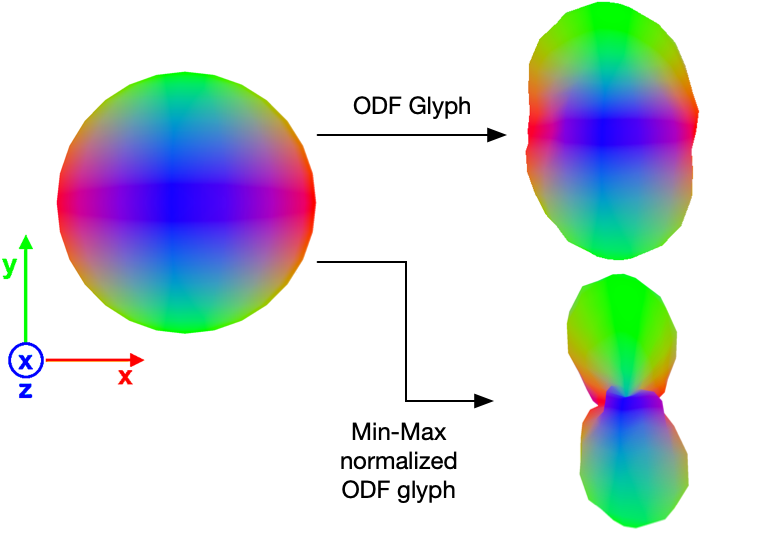
\includegraphics[width=1.00\linewidth, angle=0]{figs/SphericalMeshModulation.png}
    \caption{Glyphs obtained by modulating a sphere. The result in the upper right shows the glyph generated from its respective ODF. The image in the bottom right shows the glyph generated by a min-max normalized version of the ODF, which has a more pronounced orientational structure. The color scheme is describe in the equation \ref{eq::glyph_color}}
    \label{fig::intro_glyph}
\end{figure}

%\sout{These advanced methods that requires a HARDI acquisition, which will be called in this work as HARDI methods, aims to reconstruct} \textcolor{blue}{Tuch showed that when the angular acquisitions are uniform, one can synthesize from the samples} an orientation distribution function (ODF) that represents the diffusion process. \sout{Some of them are}\textcolor{blue}{This function is} model-free\sout{, which}\textcolor{blue}{It} estimates the diffusion displacement from the Fourier relation between the DW-MRI signal to its respective diffusion displacement \cite{TuchQBall2004, wedeen2005,  yeh2010}\sout{ and others are}\textcolor{blue}{Tournier presented a} model-based \textcolor{blue}{approach}\todo{It is not clear the underlying model! FOD, fiber orientation density???}\textcolor{red}{, where they model the underlying fiber signal obtained by its respective decay on the diffusion acquisition \cite{tournier2007}.}

%\sout{These advanced methods that requires a HARDI acquisition, which will be called in this work as HARDI methods, aims to reconstruct} \textcolor{blue}{Tuch showed that when the angular acquisitions are uniform, one can synthesize from the samples} an orientation distribution function (ODF) that represents the diffusion process. \sout{Some of them are}\textcolor{blue}{This function is} model-free\sout{, which}\textcolor{blue}{It} estimates the diffusion displacement from the Fourier relation between the DW-MRI signal to its respective diffusion displacement \cite{TuchQBall2004, wedeen2005,  yeh2010}\sout{ and others are}\textcolor{blue}{Tournier presented a} model-based \textcolor{blue}{approach}\todo{It is not clear the underlying model! FOD, fiber orientation density???}\textcolor{red}{, where they model the underlying fiber signal obtained by its respective decay on the diffusion acquisition \cite{tournier2007}.}

%An ODF consists in an association of a set of directions, each one of \sout{them}\textcolor{blue}{which} \textcolor{blue}{is} represented by a unity vector $\bm{u}$, to a scalar $\psi(\bm{u})$. The most common approach to represent an ODF by a glyph is through the spherical polar plot. In this category of a glyph, a \todo{Reference to normalized ODF}normalized \sout{version of the} ODF deforms a sphere accordingly to \sout{the equation}\textcolor{blue}{Eq.} \ref{eq::normglifo}:

\begin{equation}
\label{eq::normglifo}
    R(\bm{u}) = \frac{\psi(\bm{u}) - min(\psi(\bm{u}))}{max(\psi(\bm{u})) - min(\psi(\bm{u}))}
\end{equation}

%where $R(\bm{u})$ is the length of a deformed sphere in the direction $\bm{u}$.

These glyphs provide a clear visualization of local diffusion through its ODF samples. Researchers use them to validate imaging methods \cite{descoteaux2007_QBI,  TuchQBall2004,tournier2007,Tournier2004DirectEO, tuch2002,  yeh2010} and assess the local relationship between the acquisition quality, the imaging method, and the underlying fiber orientation distribution (FOD) computed \cite{cho2008, daducci2014,descoteaux2007,  vega2009}. %The FODs extracted from an imaging method applied to a DWI acquisition are used as input of fiber tracking algorithms. %The conjecture of the possibility of brain connectivity from the DWI acquisitions motivates this research area's main motivation.

%\todo{Insert a figure to help in understanding.}These glyphs\textcolor{blue}{, as illustrated in Fig~\ref{???},} \sout{give}\textcolor{blue}{provide} a clear visualization of local \sout{information in} diffusion \sout{imaging methods} \textcolor{blue}{in each voxel}. \sout{It is used by} \todo{References?}Researchers use them to \todo{???}\textcolor{red}{assess the acquisition quality,} \sout{attest the validity of}\textcolor{blue}{validate} an imaging method, \sout{the adequability of it given an acquisition} and \sout{the} check the relationship between the \textcolor{blue}{applied} imaging method \sout{used with} \textcolor{blue}{and the} fiber reconstruction algorithms called tractography.

Color can enhance the orientation information, making its spatial direction explicit. A simple color mapping is applied to highlight a diffusion vector $\bm{u}$ in three orthogonal directions, as defined in Eq. \ref{eq::glyph_color}.

\begin{equation}
\label{eq::glyph_color}
    (r,g,b) = (|u_x|,|u_y|,|u_z|)
\end{equation}

In the brain anatomical axes, the red color represents the mediolateral direction, the green refers to the anteroposterior direction, and the blue, inferior-superior direction. The DWI community commonly uses this color scheme.

%\todo[inline]{I suggest writing motivation to this work: the challenging remaining problems and the one you are supposed to solve.}

In this work, we present an interactive GPU-accelerated polygon-based rendering scheme of multiple spherical polar plots from ODF samples. We applied instance rendering to reduce the CPU-GPU data traffic.%\sout{The gains of performance are given by decreasing the amount of data traffic CPU-GPU by taking out redundant information on each drawing request. This is achieved by using instance rendering.}

%In this work, we present a\textcolor{blue}{n interactive GPU-accelerated} rendering scheme \sout{that aims to, given samples of ODFs associated with a spherical mesh, we} \textcolor{blue}{to} render a set of spherical polar plot\textcolor{blue}{s from ODF samples}. \textcolor{blue}{Inspired by Voltoline and Wu's work, we applied instance rendering and transform feedback to reduce the CPU-GPU data traffic.}\sout{The gains of performance are given by decreasing the amount of data traffic CPU-GPU by taking out redundant information on each drawing request. This is achieved by using instance rendering.}

This rendering scheme, integrated with visualization systems to diffusion images, can be a powerful tool for researchers in the area to assess a set of local diffusion profiles and improve their understanding of advanced methods for diffusion imaging.

This paper is divided in \ref{sec::conclusions} sections. In section \ref{sec::related_work}, we discuss the related works; in the section \ref{sec::odf_glyph_rendering}, we discuss the rendering scheme, the data structures associated, an overview of the GPU shaders, and an optimization strategy for symmetrical ODFs; in the section \ref{sec::results}, we analyze the glyphs generated and show performance measurements; and in the section \ref{sec::conclusions}, we conclude the work.

%\todo{Redundant text. Instead, write the expected contribution.}\sout{The integration of this rendering scheme in a DW-MRI visualization can be  It improves the understanding of the output result of an diffusion imaging method applied to DW-MRI, as well as provide an a visual information of the underlying model where directional information of fibers is extracted to be used on brain fiber reconstruction. The real time factor can improve the visual interactivity of the research in the area.}



%We ask authors to follow this guideline and make paper look exactly like as this document. The easiest way to do this is simply to download a template from \cite{jou01a} and replace the content with your own.

%\section{Background}



\section{Related work}
\label{sec::related_work}

%\todo[inline]{You must show why the works are related to your work. Which aspects did you take advantage of in your work?}



%Polygons based glyph rendering schemes is an area that has not been much explored by the HARDI community. Shattuck et al. \sout{\cite{shattuck2008} showed results of a polygon based approach} \textcolor{blue}{presented} in \sout{his}\textcolor{blue}{their} work \textcolor{blue}{\cite{shattuck2008} the rendering of ODFs as spherical meshes of 225 vertices and 2 million triangles in 10 FPS.}\sout{ and, at that time, the result reported by them was 10 FPS when using a spherical mesh of 225 vertices, with 2 million triangles being rendered.} The authors \sout{do}\textcolor{blue}{did} not \sout{explain} detail\sout{ed} their rendering scheme\sout{ and imply that they were not programming the GPU. It is worth mentioning that instance rendering was not released back then}.



Polygons-based glyph rendering schemes are an area that has not been much explored by the HARDI community. Shattuck et al. \cite{shattuck2008} presented the rendering of these glyphs and reports a limitation in the rendering performance. The performance result reported by them were 10 FPS for a spherical mesh of 225 vertices and 2 million triangles being rendered. The authors did not detail their rendering scheme and did not take advantage of the GPU programming to improve it, as we show in this work.
%ALGO RELEVANTE: ESSE TRABALHO DO SHATTUCK É O ÚLTIMO DA ÁREA QUE TEM ALGUMA COISA A VER COM O MEU, QUE É RENDERIZAR GLIFOS HARDI EM TEMPO REAL VIA POLIGONOS.


% \sout{ and imply that they were not programming the GPU. It is worth mentioning that instance rendering was not released back then}.

Peeters et al. \cite{peeters2009} proposed a ray casting approach to render glyphs as an alternative to the polygon-based previous works and achieved better performance results by comparing with the approach of Shattuck et al. \cite{shattuck2008}. In their approach, each glyph's CPU-GPU data traffic consists of coefficients of spherical harmonics for a GPU-based ray casting algorithm.

%They also compared their approach to the polygon based rendering scheme proposed by Shattuck et al. \cite{shattuck2008}. 

Voltoline et al. \cite{voltoline2021} proposed a real-time rendering scheme for a glyph representation of diffusion tensor called superquadrics \cite{Kindlmann2004}. In their work, they minimize the CPU-GPU data traffic to a few parameters that customize the glyphs in each drawing request using the instance rendering technique, obtaining interactive performance results. These results influenced us to adapt their scheme in our HARDI glyph rendering scheme.

%\todo[inline]{It is important to cite Voltoline's work.}

%\section{Rendering scheme}
\section{ODF Glyph Rendering}
\label{sec::odf_glyph_rendering}

Our goal is to show the rendering scheme of the glyphs to be shown in the scene. The subsection \ref{ssec::precomputation} describes the procedures that must be done at the initialization of the rendering scheme; in the subsection \ref{ssec::datastruct}, we describe the input data structures that customize the glyphs and are the most of the CPU-GPU data traffic and an optimization for symmetrical ODFs; in the subsection \ref{ssec::rendering}, we provide a summary of the CPU and GPU division of tasks.% and, in the subsection \ref{ssec::optimization}, we discuss an optimization that can be done in symmetrical ODFs.

%The input of the rendering scheme consists in two set of elements: the set positions in the scene and a set of ODF profiles that .

%We divide the rendering scheme in precomputation and drawing request. The precomputation  refers to the part of the rendering scheme that is done at the beginning of scheme and only once, and the 

%\todo[inline]{An overview of the proposal. It could be a flowchart}

\subsection{Initialization}
\label{ssec::precomputation}

%The glyphs consist of spheres with each one of its radius points deformed by its respective ODF value.

The scheme's initialization consists on the setup of a mesh of a unit sphere centered in the origin with N points set $\Pi = \{P_1, P_2, \dots, P_N\}$. The mesh is sent to the GPU with non repeated points, along with its respective index buffer, only once as an attribute to be instanced.



%\todo[inline]{What to be rendered? At least a paragraph explaining the objects to be rendered. Spheres deformed by ODFs?}

%\begin{enumerate}
    %\item Compute spherical mesh and its index buffer and send to GPU.
    %\item Compute matrix $\bm{\Psi}$ and send to GPU as a texture.
%\end{enumerate}


\subsection{Data Structures}
\label{ssec::datastruct}

Two elements customize each one of the glyphs: ODF samples and their position. These elements are sent to the GPU in every draw request.

First, let us define the vector set $\Upsilon$ as a function of $\Pi$ as shown in Eq. \ref{eq::u_vector_set}. The glyph geometry is deformed by scaling each point $P_k$ in the mesh to ODF value $\psi(\bm{u}_k)$ before translating it. The translation matrix places the deformed spherical mesh to be centered at a point $C(x, y, z)$.

\begin{equation}
\label{eq::u_vector_set}
\Upsilon = \{\bm{u}_k | \bm{u}_k = \frac{P_k - O}{|P_k - O|}, 
\begin{tabular}{@{}c@{}}
\small{$\forall P_k \in \Pi; O$ is the origin} \\
\small{and center of the sphere}

\end{tabular}
\text{ }\}
\end{equation}

%\forall P_k \in \Pi ; O \text{ is the origin } \\
%\text{}

Due to the large amount of data sent to the GPU in the drawing requests, the goal of this subsection is to show a way to organize the data in the CPU, how to send it to the GPU, and how the GPU shaders read it, so the CPU-GPU data traffic is as minimum as possible. %In this subsection, we are going to describe the general data structures of the data and in the subsection \ref{ssec::optimization}, we present an optimization of the scheme for ODFs that have symmetry.



%The rendering scheme consists of instantiating an unit radius spherical mesh of N vertices centered on the origin and sent to the GPU only once. \todo{Should the translation matrix and ODF be sent to the GPU?}\textcolor{red}{At each instance, the mesh is transformed by a translation matrix and its ODF samples.}

%The translation matrix \sout{positions}\textcolor{blue}{places} the center of the spherical mesh to \sout{its respective position}\textcolor{blue}{the center of the corresponding voxel}. The ODF samples represent the diffusion profile\textcolor{blue}{s} that are particular to each glyph. \sout{These which determines t}\textcolor{blue}{T}he \textcolor{blue}{glyph geometry}\sout{shape of the glyph} \textcolor{blue}{is reshaped} by multiplying the \textcolor{blue}{mesh normal $\bm{n}$} \sout{vertex of the mesh associated with the direction of diffusion} to \sout{its}\textcolor{blue}{the} ODF value \textcolor{blue}{whose diffusion direction is parallel to $\bm{n}$}.

%\sout{In this rendering scheme, the set consisting of the translation matrices and the ODF profiles consists are sent from the CPU to the GPU in each drawing request. Hence, in order to achieve the goal of interactivity, it is desirable that the data traffic between both parts is as little as possible.}

\subsubsection{Translation}
Let P be the number of instances of the rendering scheme and glyphs to be drawn. The translation points are organized as a vector of points $[C_1,C_2, \dots, C_P]$, where $C_i = (x_i, y_i, z_i)$, and sent to the GPU as an attribute. Each point of this attribute is unique for each one of the P instances of the spherical mesh.

%The i-th index of the matrices set vector refers to the spherical mesh's i-th instance to be rendered centered at the point $C_i(x_i, y_i, z_i)$.


%\todo[inline]{How to transfer data?}
%\sout{The traffic CPU-GPU that refers to the translation consists of sending a vector containing} \textcolor{blue}{the set of} P translation matrices as \todo{uniform array? Use the GPU/OpenGL vocabulary to make understanding easier.}\textcolor{red}{an attribute, which is unique for each spherical mesh instantiated}.

\subsubsection{ODFs}

The ODF data sent to GPU consists of the N samples referring to the diffusion profiles for each P glyphs to be drawn. We construct a $\bm{\Psi}_{PxN}$ matrix, where P is the number of glyphs to be drawn, and N is the number of samples of ODF used, as given in Eq. \ref{eq::Psi}:

\begin{equation}
\label{eq::Psi}
\bm{\Psi} = 
\begingroup % keep the change local
\setlength\arraycolsep{2pt}
\begin{bmatrix} 
    \psi_1(\bm{u}_1) & \psi_1(\bm{u}_2) & \cdots \psi_1(\bm{u}_{N-1}) & \psi_1(\bm{u}_{N})  \\    
     \psi_2(\bm{u}_1)& \psi_2(\bm{u}_2) & \cdots \psi_2(\bm{u}_{N-1}) & \psi_2(\bm{u}_{N}) \\
    \vdots & \vdots & \vdots & \vdots  \\    
     \psi_P(\bm{u}_1)&\psi_P(\bm{u}_2) & \cdots \psi_P(\bm{u}_{N-1}) & \psi_P(\bm{u}_{N})
\end{bmatrix}, 
\endgroup
\end{equation}

where $\psi_{ij}$ refers to the ODF value $\psi_i(\bm{u}_j)$ of the i-th glyph associated with the direction $\bm{u}_j$, which scales the $P_j$ vertex of the spherical mesh. The $\bm{\Psi}_{PxN}$ matrix is sent to the GPU as a 2D texture.

On the GPU, the access of ODFs to deform its respective sphere point is done by accessing the texture data through its instance and vertex indexes in the vertex shader.

The instance index (Instance\_ID) corresponds to an instanced spherical mesh centered in its respective point $P$, and since ODFs samples of one glyph are stored in the rows of $\bm{\Psi}$, the Instance\_ID access this dimension.

The vertex index (Vertex\_ID), in its turn, indicates a point of the spherical mesh, which corresponds to the column of its respective ODF value in $\bm{\Psi}$.

Hence, we perform the GPU access by a single lookup of the texture texel\footnote{In OpenGL, the lookup is done by the command texelFetch($\bm{\Psi}$, ivec2(gl\_InstanceID, gl\_VertexID), 0)[0]} using the Vertex\_ID and Instance\_ID pair. Fig.\ref{fig::GPU2glyph} illustrates the ODF access for each instance and vertex in the GPU.

%(MESMO PARÁGRAFO ACIMA, COM INDICAÇÕES OPENGL)The access in the GPU of ODFs to deform its respective sphere point is done by accessing the texture data through its instance and vertex indexes in the vertex shader. To achieve this, it is necessary that the vertex index (Vertex\_ID) (gl\_VertexID\footnotemark) of the direction of each vertex correspond to the column of its respective ODF value $ \psi (\bm{u}_j) $ in diffusion profile matrix. The access of the rows of the diffusion profile matrix, corresponding to the diffusion profiles in its respective point is accessible by the instance index (gl\_InstanceID\footnotemark [\value{footnote}]). Having the data organized in this established way, the access is done by perfoming a single lookup of the texel in the texture using the Vertex\_ID and Instance\_ID as a pair. In OpenGL, this can be done by the function texelFetch\footnotemark[\value{footnote}] with the row and column access arguments through the pair ( gl\_VertexID, gl\_InstanceID)\footnotemark [\value{footnote}] \footnotetext{All commands refer to OpenGL API and GLSL shading language.}. How to access the GPU of the profile matrix is illustrated in the Fig.\ref{fig::GPU2glyph}.

%\todo[inline]{It is not understandable the caption!!! And it is not clear what is exactly the column and what is the row. It seems that your texture is 3D. columen (vertex\_ID), row (instance\_ID), depth (diffusion profile consisting of a series of values).}

\begin{figure}[htb]
    \centering
    %\rule{6cm}{3cm}
    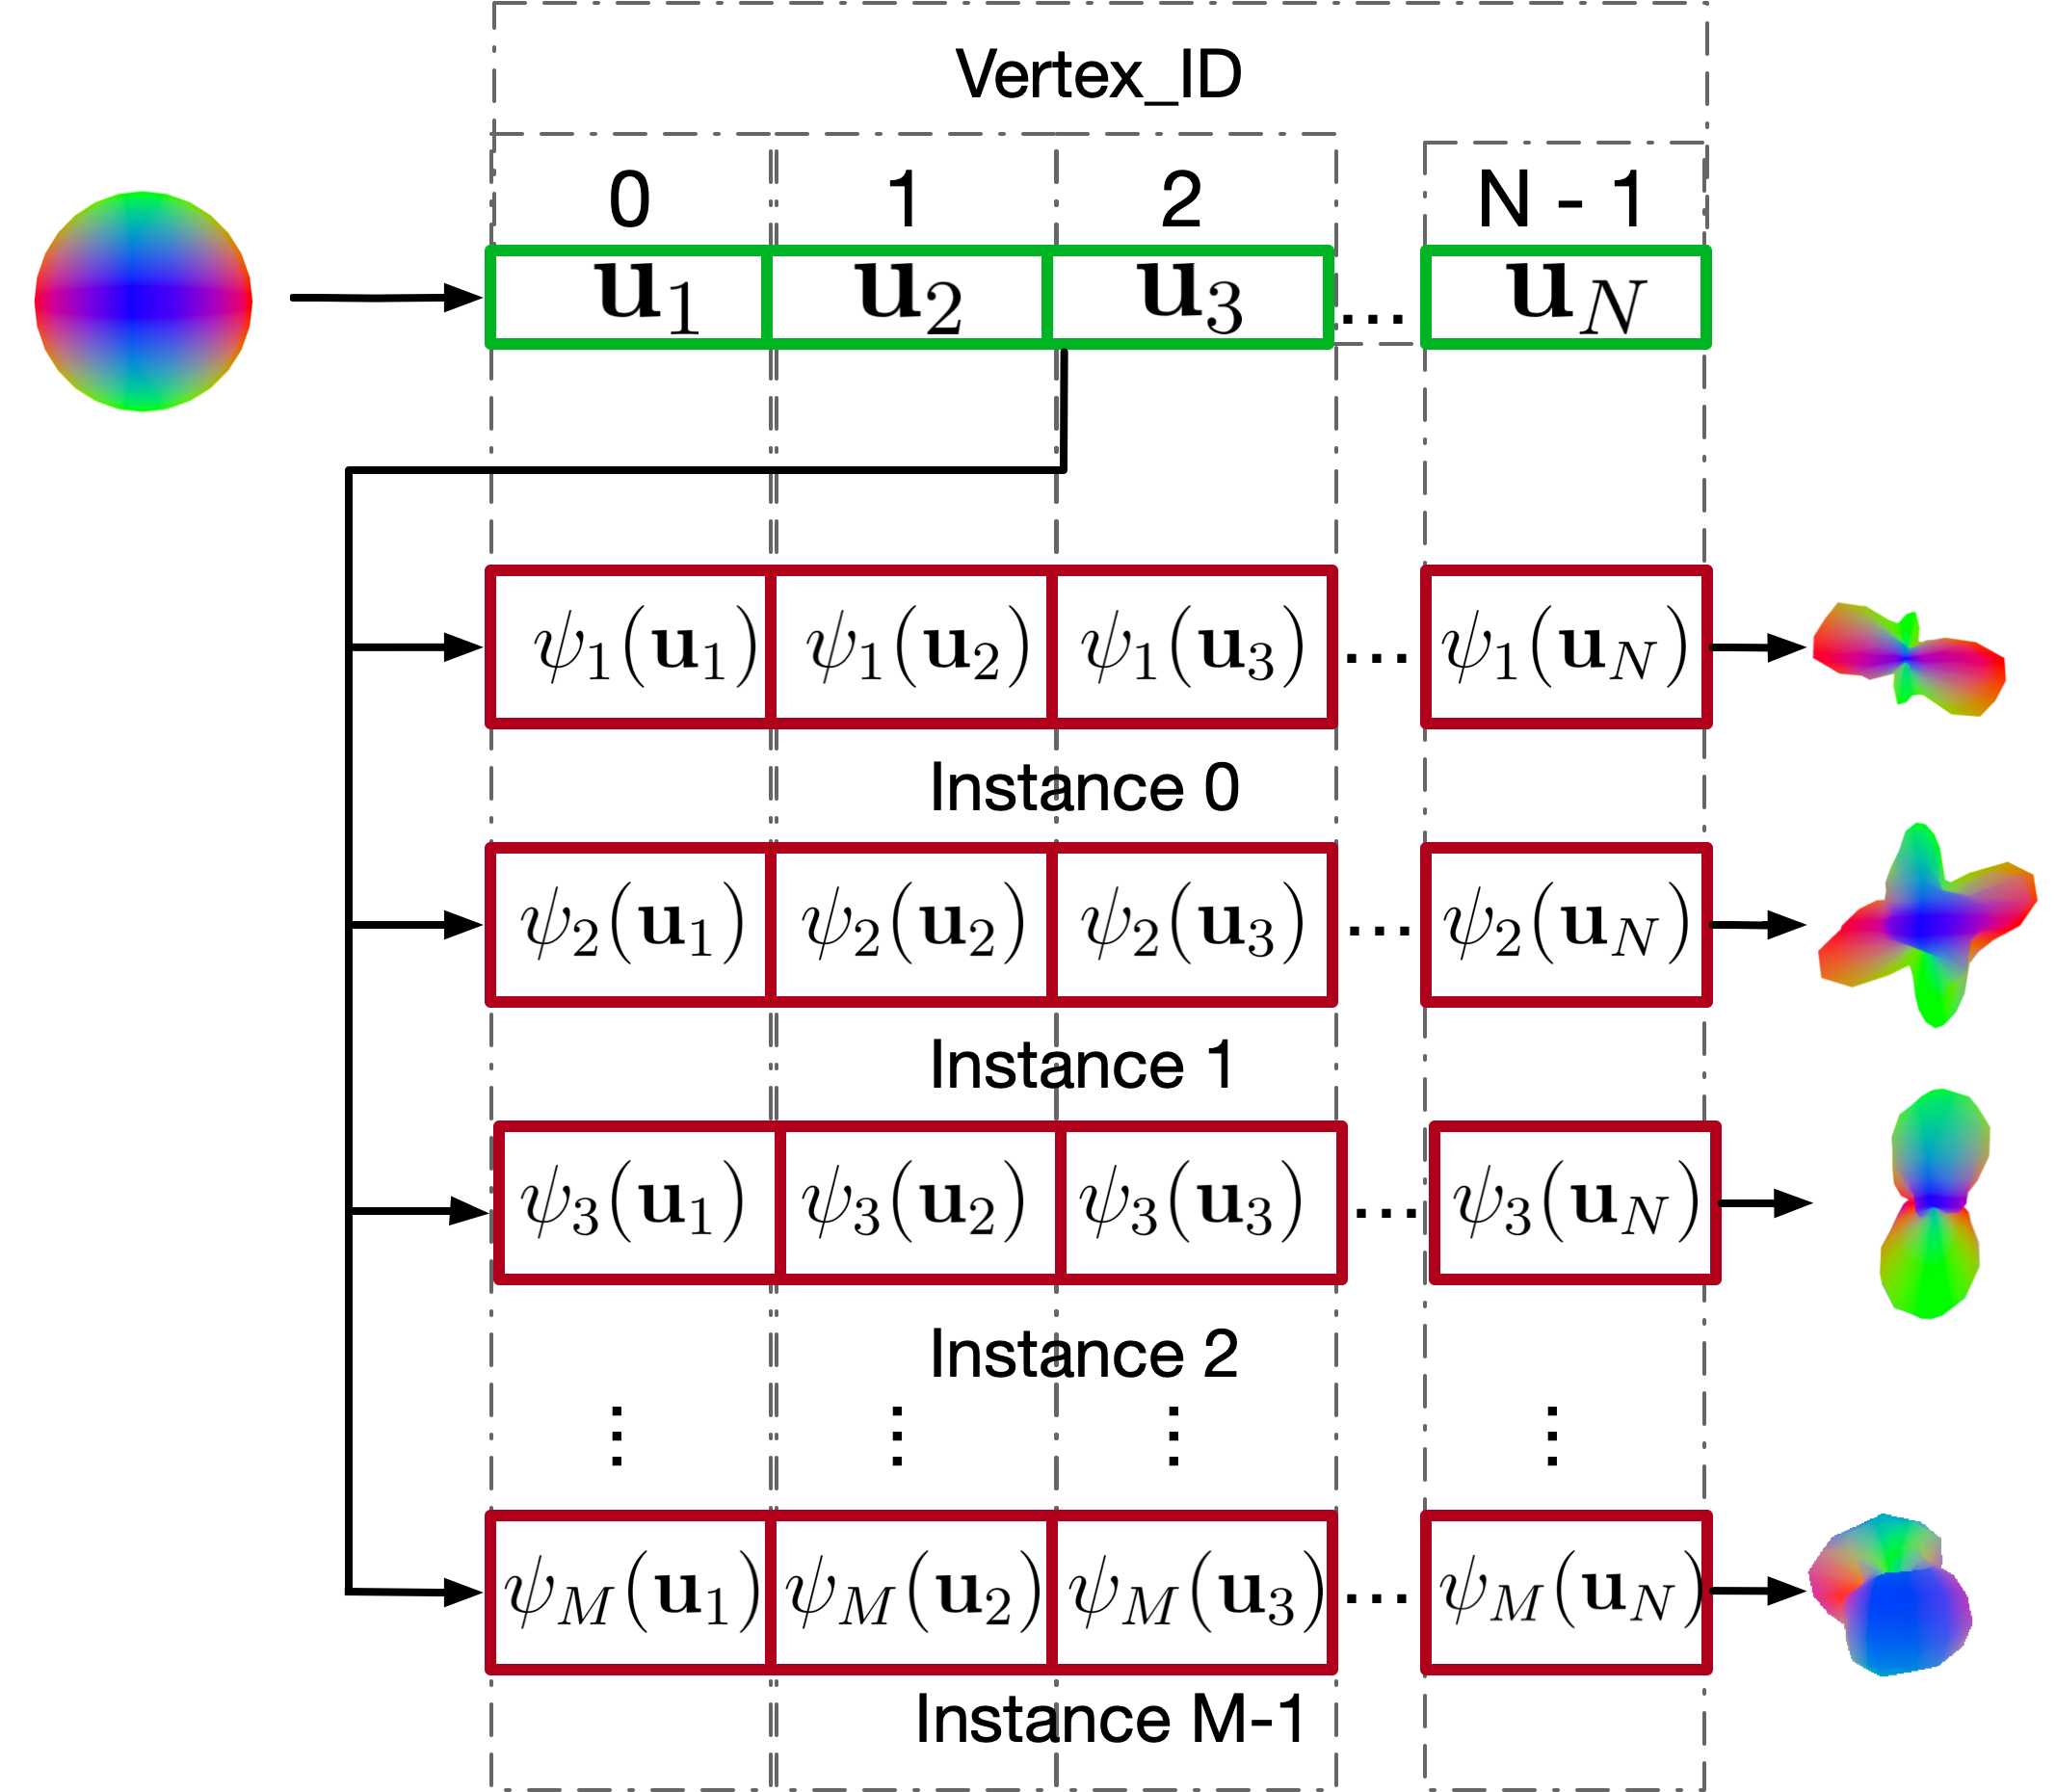
\includegraphics[width=1.0\linewidth, angle=0]{figs/rendering_scheme/GPU2Glyph.png}
    \caption{
    Illustration of $\bm{\Psi}$ (in red) and its lookup procedure in the vertex shader by its Vertex\_ID and instance indexes for $P$ glyphs to be rendered. The data structure of $\Upsilon$ is in green. For an ODF $\psi_i(\bm{u})$, the value recovered for each $u_k$ scales its respective mesh point $P_k$, deforming it.
    %\textcolor{red}{Illustration of the data organization in the GPU of the profile matrix (red) sent as 2D-Texture. The vertices of the spherical mesh are in green. At each instance, the customization of the glyph occurs through the multiplication of the mesh vertex with its respective value, recovered in the vertex shader through its vertex index for the P glyphs to be rendered}.
    }
    \label{fig::GPU2glyph}
\end{figure}

%\section{Scheme Overview}
%\label{sec::scheme_overview}
%\subsection{Precomputation}
%\begin{enumerate}
%    \item Compute spherical mesh and its index buffer and send to GPU.
%\end{enumerate}
%\subsection{CPU}
%\begin{enumerate}
%    \item Compute matrix $\bm{\Psi}$ and send to GPU as a texture.
%\end{enumerate}
%\subsection{GPU}
%\subsubsection{Vertex Shader}
%\begin{enumerate}
%    \item Lookup the coefficient that customize the glyphs and multiply by the spherical vertex;
%    \item perform translation of the glyph;
%    \item do scaling and camera related transformations;
%    \item compute color as a function of the spherical mesh vertex accordingly to equation %\ref{eq::glyph_color} and send to fragment shader.
%\end{enumerate}
%\subsubsection{Fragment Shader}
%\begin{enumerate}
%    \item Set the output color as the rasterized color defined in the vertex shader.
%\end{enumerate}

\subsubsection{Optimization on symmetrical ODFs}
\label{sssec::optimization}

In this subsection, we show an adaption of the data structure described in the subsection \ref{ssec::datastruct} to symmetrical ODFs and a strategy to decrease its related CPU-GPU data traffic by half.

An ODF is symmetrical if $\psi(\bm{u}) = \psi(-\bm{u})$ for all $\bm{u}$ in the unit sphere. This symmetry applies to the diffusion behavior, which makes this section entirely applicable for rendering HARDI ODFs.%This property is present on all imaging methods for diffusion.

Firstly, we suggest the use of a symmetrical spherical mesh. That means, if a point $P \in \Pi \implies -P \in \Pi$ as well. As an example, a mesh generated by any order of a tessellated icosahedron fits this criterion.

Secondly, we recommend that the chosen symmetrical spherical mesh's data structure is organized so that a point $P$ in an even index is followed by $-P$. This spherical mesh is sent to the GPU in the same form as stated in the subsection \ref{ssec::precomputation}.

%\textcolor{red}{Firstly, we suggest the use of a symmetrical spherical mesh, which can be, for example, any order of a sphere \todo{How? It must be explained!}generated by a tessellated icosahedron. We suggest as well that the vector containing its vertices is organized in such a way that the vector in the (2k)-th index is symmetrical to the (2k+1)-th.}

Following these recommendations, the data structure of points in the sphere $[P_1, P_2, P_3, P_4, \dots, P_{N-1}, P_N]$ becomes $[P_1, -P_1, P_3, -P_3, \dots, P_{N-1}, -P_{N-1}]$ and their associated $\Upsilon$ turns to $[\bm{u}_1, -\bm{u}_1, \bm{u}_3, -\bm{u}_3, \dots, \bm{u}_{N-1}, -\bm{u}_{N-1}]$. In this situation, $\bm{\Psi}$ is now:

\begin{equation*}
\bm{\Psi} = 
\begingroup % keep the change local
\setlength\arraycolsep{2pt}
\begin{bmatrix} 
    \psi_1(\bm{u}_1) & \psi_1(-\bm{u}_1) & \cdots \psi_1(\bm{u}_{N-1}) & \psi_1(-\bm{u}_{N-1})  \\
    
     \psi_2(\bm{u}_1)& \psi_2(-\bm{u}_1) & \cdots \psi_2(\bm{u}_{N-1}) & \psi_2(-\bm{u}_{N-1}) \\

    \vdots & \vdots & \vdots & \vdots  \\
    
     \psi_P(\bm{u}_1)&\psi_P(-\bm{u}_1) & \cdots \psi_P(\bm{u}_{N-1}) & \psi_P(-\bm{u}_{N-1})
    
\end{bmatrix},
\endgroup
\end{equation*}

where each of the (2k+1)-th column is the same as the (2k+2)-th ($0 \leq k < \frac{N}{2}$).

Hence, we define a matrix $\bm{\Psi^h}_{Px\frac{N}{2}}$ such that $\bm{\psi^h}_{ij} = \bm{\psi}_{i(2j-1)}$, which is described in the expression below:

%\todo{Very confusing!}We \textcolor{blue}{re}define \textcolor{blue}{Eq. \ref{eq::Psi}}, \sout{a matrix $\bm{\Psi^h}_{Px\frac{N}{2}}$ where} \textcolor{blue}{such that} $\bm{\psi^h}_{ij} = \bm{\psi}_{i(2j-1)}$. \sout{that is sent to GPU on every drawing request. Its form is stated below:}\textcolor{blue}{It assumes the form}

\begin{equation*}
\label{eq::Psi_changed}
\bm{\Psi^h} = 
\begingroup % keep the change local
\setlength\arraycolsep{2pt}
\begin{bmatrix} 
    \psi_1(\bm{u}_1) & \psi_1(\bm{u}_3) & \cdots \psi_1(\bm{u}_{N-3}) & \psi_1(\bm{u}_{N-1})  \\
    
     \psi_2(\bm{u}_1)& \psi_2(\bm{u}_3) & \cdots \psi_2(\bm{u}_{N-3}) & \psi_2(\bm{u}_{N-1}) \\

    \vdots & \vdots & \vdots & \vdots  \\
    
     \psi_P(\bm{u}_1)&\psi_P(\bm{u}_3) & \cdots \psi_P(\bm{u}_{N-3}) & \psi_P(\bm{u}_{N-1})
    
\end{bmatrix}
\endgroup
\end{equation*}

$\bm{\Psi^h}$ is sent to the GPU in the drawing requests in the same way as $\bm{\Psi}$ described in the subsection \ref{ssec::datastruct} and the difference lies in the lookup process. On the GPU, the vertices corresponding to the 2k-th and (2k+1)-th Vertex\_ID in the spherical mesh of the same instance have the same value to lookup\footnote{In OpenGL, the lookup is done by the command texelFetch($\bm{\Psi^h}$, ivec2(gl\_InstanceID, gl\_VertexID/2), 0)[0]}, corresponding to the k-th column, which can be accessed accordingly in the vertex shader.

%\sout{In}\textcolor{blue}{On} the GPU, the  in $\bm{\Psi}^h$, which corresponds to the K-th index of the matrix, which can be accessed accordingly in the vertex shader.



\subsection{GPU Rendering Overview}
\label{ssec::rendering}

\subsubsection{Vertex Shader}
\begin{enumerate}
    \item Lookup the coefficient that customizes the glyphs and multiply by the spherical vertex;
    \item perform translation of the glyph;
    \item scale and apply the model-view-projection transformation;
    \item compute color as a function of the spherical mesh vertex accordingly to Eq. \ref{eq::glyph_color} and send to the fragment shader.
\end{enumerate}
\subsubsection{Fragment Shader}
\begin{enumerate}
    \item Set the output color as the rasterized color set in the vertex shader.
\end{enumerate}


%\section{Optimization}

%\todo[inline]{Is it not better to put together with other part of description?}


\section{Results}
\label{sec::results}

\subsection{Visual aspects}

Fig. \ref{fig::ex_glyph} shows glyphs for different meshes. One can see that a spherical mesh defined by an $8^{th}$ (Fig. \ref{fig::ex_glyph8}) tessellation order of the icosahedron is fine enough that does not have much visual difference compared to the $16^{th}$ order (Fig. \ref{fig::ex_glyph16}).


Fig. \ref{fig::ex_glyph_DWI_visualization} shows an application of the proposed scheme integrated into a DWI visualization system.

\begin{figure}[h]
\centering
\captionsetup[subfloat]{farskip=0pt,nearskip=0pt}
    \subfloat[4-th order (162 vertices and 320 triangles per glyph) ]{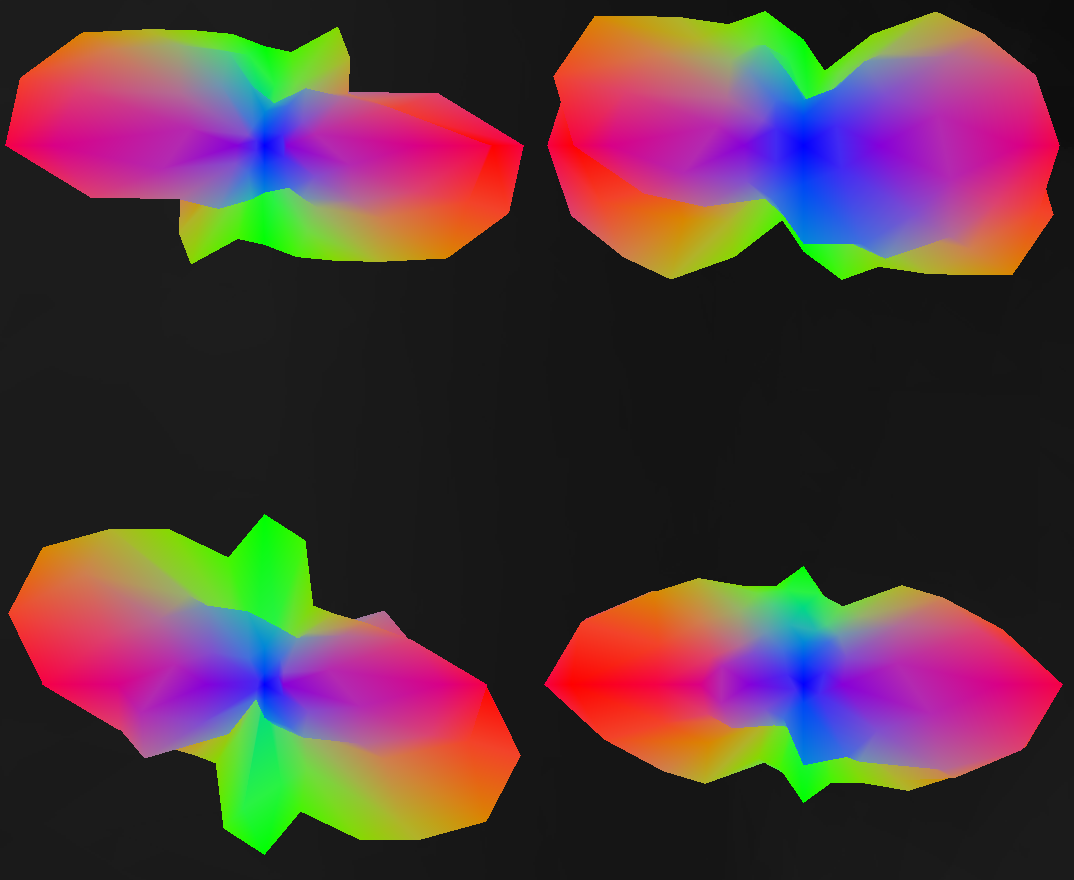
\includegraphics[width=.75\linewidth, angle=0]{figs/Results/Glyphs_4.png}
    \label{fig::ex_glyph4}
    }
    \\
    \subfloat[8-th order (642 vertices and 1280 triangles per glyph) ]{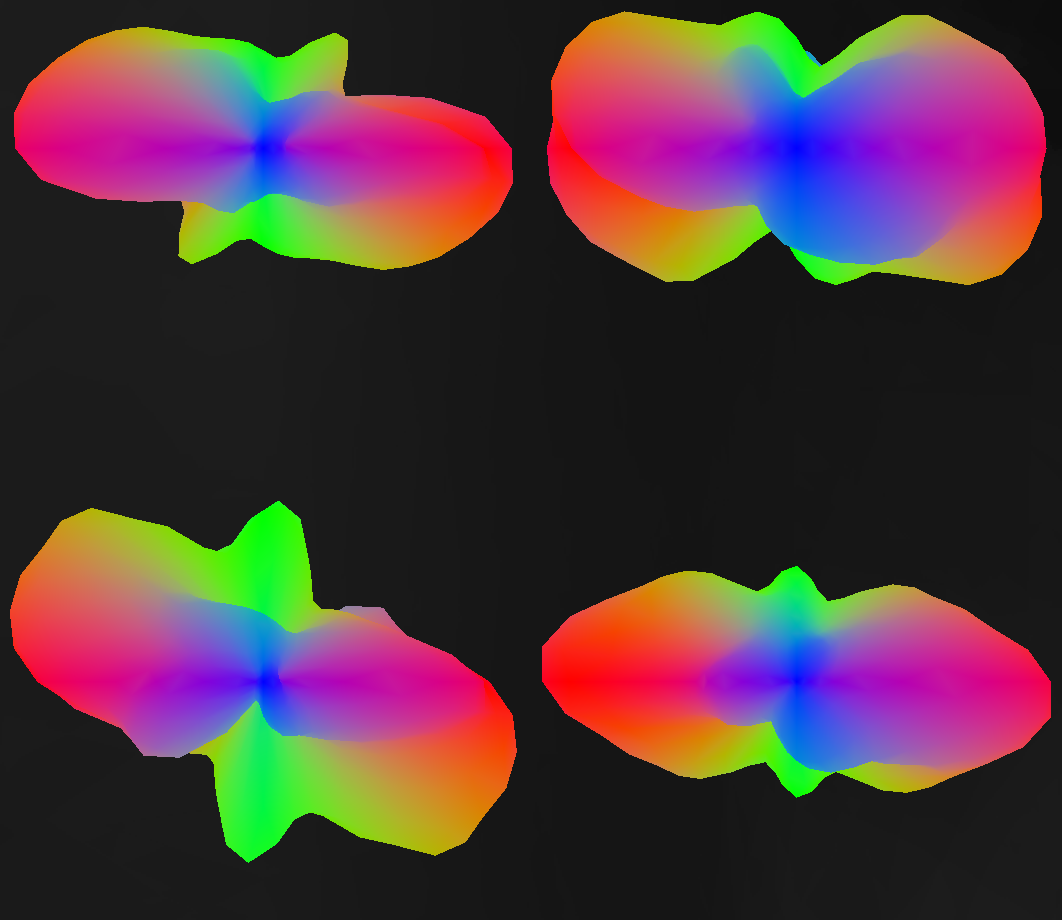
\includegraphics[width=.70\linewidth, angle=0]{figs/Results/glyphs_8.png}
    \label{fig::ex_glyph8}
    }
    \\
    \subfloat[16th order (2562 vertices and 5120 triangles per glyph)]{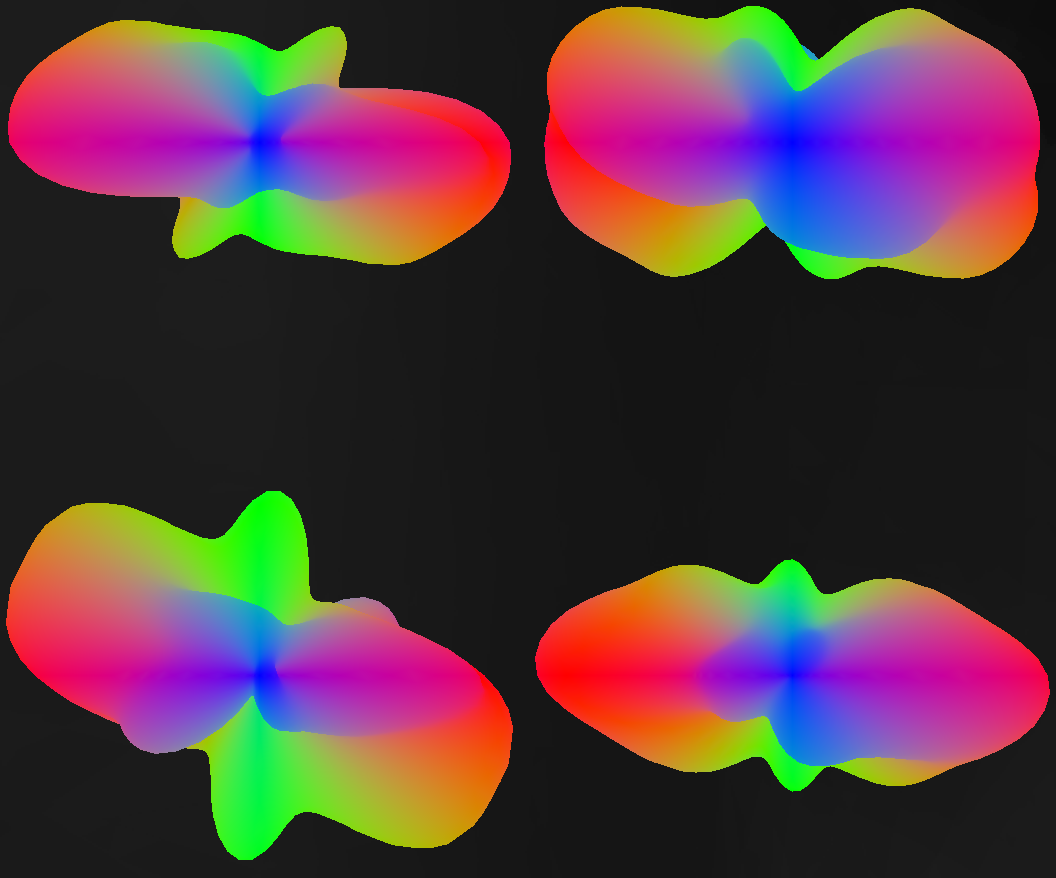
\includegraphics[width=.70\linewidth, angle=0]{figs/Results/glyphs_16.png}
    \label{fig::ex_glyph16}
    }
     \caption{Polygon based HARDI glyphs visualization for different orders of tessellation of an icosahedron. The glyphs refer to the same DWI samples. The method used to generate is the Generalized Q-Sampling Imaging (GQI) \cite{yeh2010}} %!!VER SE ISSO TA CERTO
    \label{fig::ex_glyph}
\end{figure}



%\begin{figure}[h]
    %\centering
    %\rule{6cm}{3cm}
    %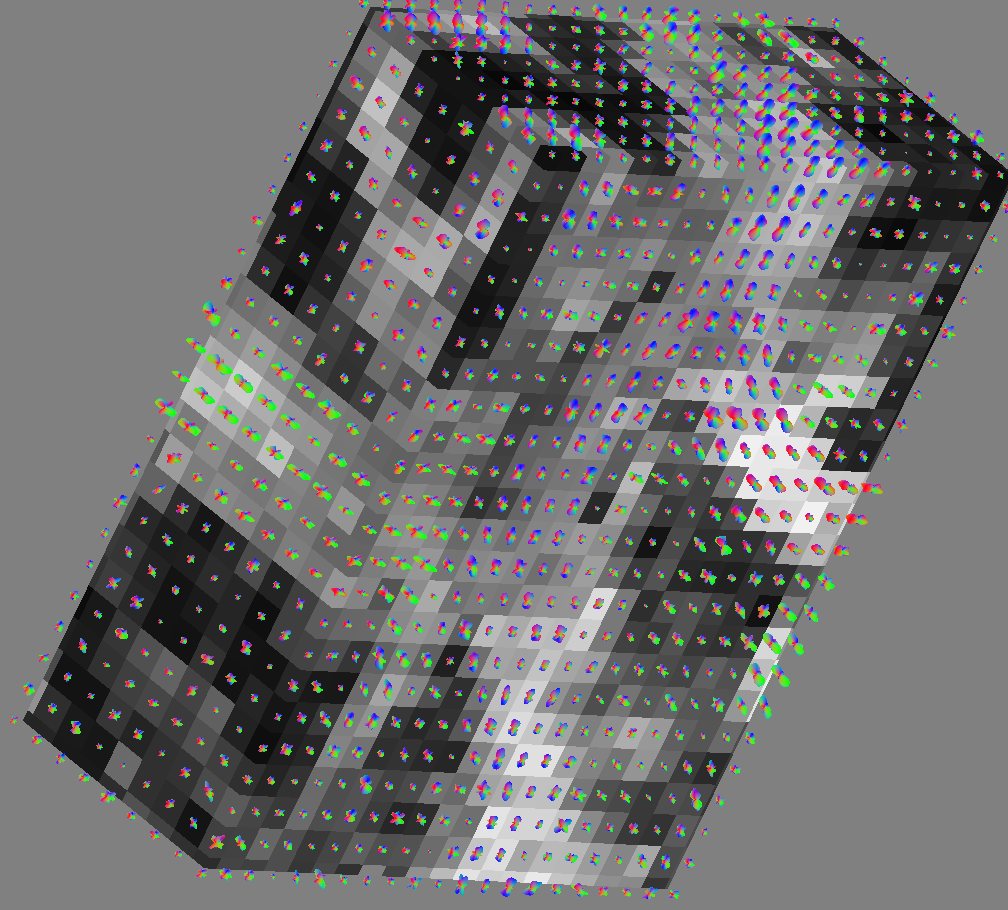
\includegraphics[width=1.00\linewidth, angle=0]{figs/Results/Glyphs_onFAMAP_2.png}
    %\caption{Glyphs integrated into a DW-MRI's fractional anisotropy map. The parallelepiped shows the region where the pyramidal tract (glyphs predominantly blue) crosses the corpus callosum (predominantly red). In the middle of the left face, the predominantly green glyphs corresponds to the region of the superior longitudinal fasciculus. The spherical mesh used corresponds to an 8-th tessellated icosahedron}
    %\label{fig::ex_glyph_FAMAP}
%\end{figure}

\subsection{Performance}

In Fig. \ref{fig::benchmark_full} and \ref{fig::benchmark_half} follows the benchmark of the rendering scheme without and with the optimization for symmetrical ODFs. The data structures setup process is accelerated by using CPU parallelism. The computer used was a Macbook Pro Retina 13' early 2015, with an Intel Core i5 Dual-Core 2.7GHz CPU, 8 GB RAM and a Intel Iris 6100 GPU with 1536 MB.


\begin{figure}[h]
\centering
\captionsetup[subfloat]{farskip=0pt,nearskip=0pt}
    \subfloat[General rendering scheme for ODFs benchmark ]{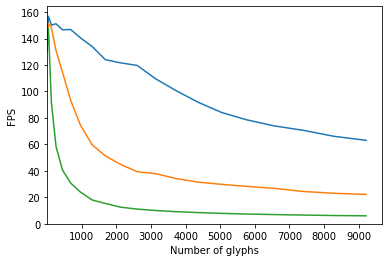
\includegraphics[width=.99\linewidth, angle=0]{figs/Benchmark/benchmark_full.png}
    \label{fig::benchmark_full}
    }
    \\
    \subfloat[Optimized rendering scheme for symmetrical ODFs benchmark ]{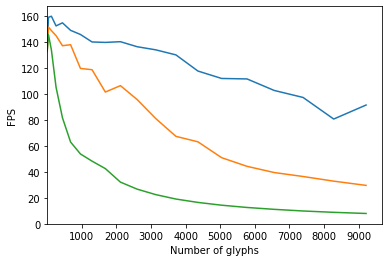
\includegraphics[width=.99\linewidth, angle=0]{figs/Benchmark/benchmark_half.png}
    \label{fig::benchmark_half}
    }
    \\
     \caption{Glyph rendering FPS $\times$ number of glyphs being rendered. The blue, orange and green curves correspond to a spherical mesh of 162, 642, 2462 vertices respectively. These meshes are generated by $4^{th}$, $8^{th}$ and $16^{th}$ order tessellation of the icosahedron} %!!VER SE ISSO TA CERTO
    \label{fig::benchmark}
\end{figure}

The results indicates that our scheme gives satisfactory results for interactive usage. Using this scheme, it is possible to render thousands of glyphs in interactive rates using a $4^{th}$ order tessellation of the icosahedron and hundreds with $16^{th}$ order, as shown in Fig. \ref{fig::benchmark_half}.

There is a relevant performance difference in the scheme by taking advantage of the ODF's symmetry. For example, in the 642 vertices spherical mesh, without optimization, the graphic hits 60 FPS with less than 2000 glyphs rendered, while taking advantage of the symmetry of ODFs makes it possible to render 4000, obtaining similar performance.




%If the ODFs are stored as coefficients of spherical harmonics, it needs a step of sampling over a spherical mesh.


%Mention comparison with raycasting methods



\subsection{Application}

In this section, we describe the implementation of the rendering scheme in a multimodal visualization environment with DWI functionalities \cite{VMTKNeuro}. In this environment, there is a ray casting based rendering for MRI/DWI volumes and a system for appearing samples detection, which is proposed and described by Voltoline et al. \cite{voltoline2021}. Fig. \ref{fig::ex_glyph_DWI_visualization} shows an result of the proposed rendering scheme applied to this environment.

\begin{figure}[h]
    \centering
    %\rule{6cm}{3cm}
    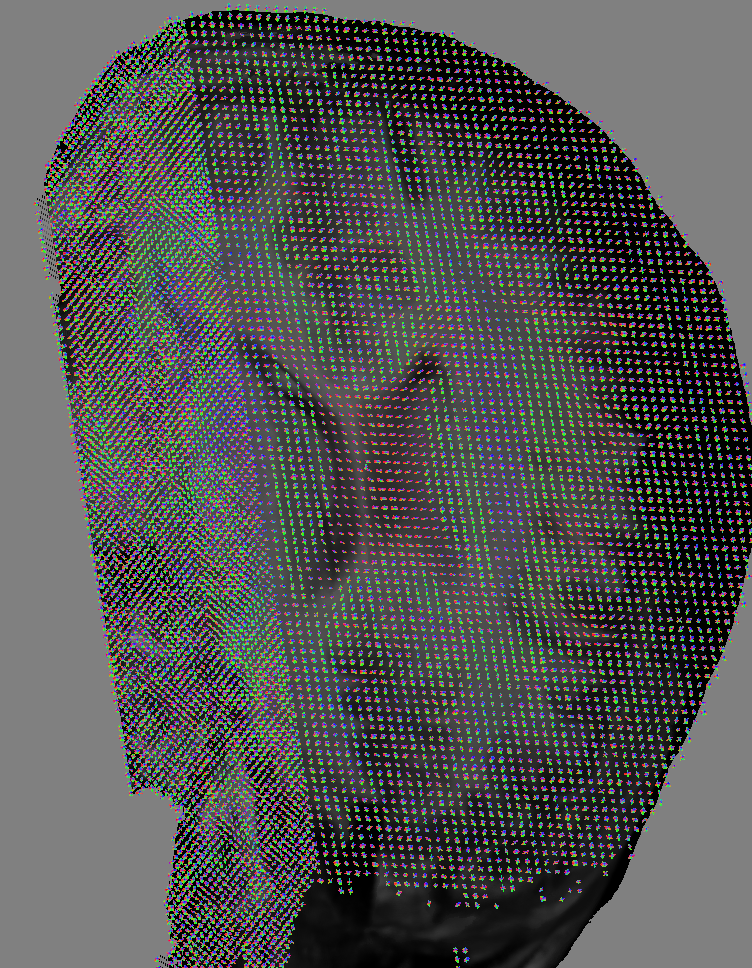
\includegraphics[width=1.00\linewidth, angle=0]{figs/Results/glyphs_integrated_DWI.png}
    \caption{Glyphs integrated into a DW-MRI's visualization scheme. The glyphs are located in a midaxial region of the brain, cutted in the left side %. The spherical mesh used corresponds to an 8-th tessellated icosahedron
    }
    \label{fig::ex_glyph_DWI_visualization}
\end{figure}

In this environment, a HARDI method is computed through its samples in a hemisphere of a spherical mesh for all voxels contained in a DWI, as well with their respectives translation coordinates to its center in the volume space. The visualization system renders the DWI volume, with the option to co-register with its respective anatomical T1 MRI. There is a functionality to detect the samples appearing on screen, returning their respective indexes of the volume. From these indexes, the buffer for the translation coordinates set and their respective HARDI data are set up to be sent to GPU as discussed in subsection \ref{ssec::datastruct}. The computation from the HARDI data to $\bm{\Psi^h}$ is illustrated in Fig. \ref{fig::vmtk_precomputed2GPU}.

\begin{figure}[h]
    \centering
    %\rule{6cm}{3cm}
    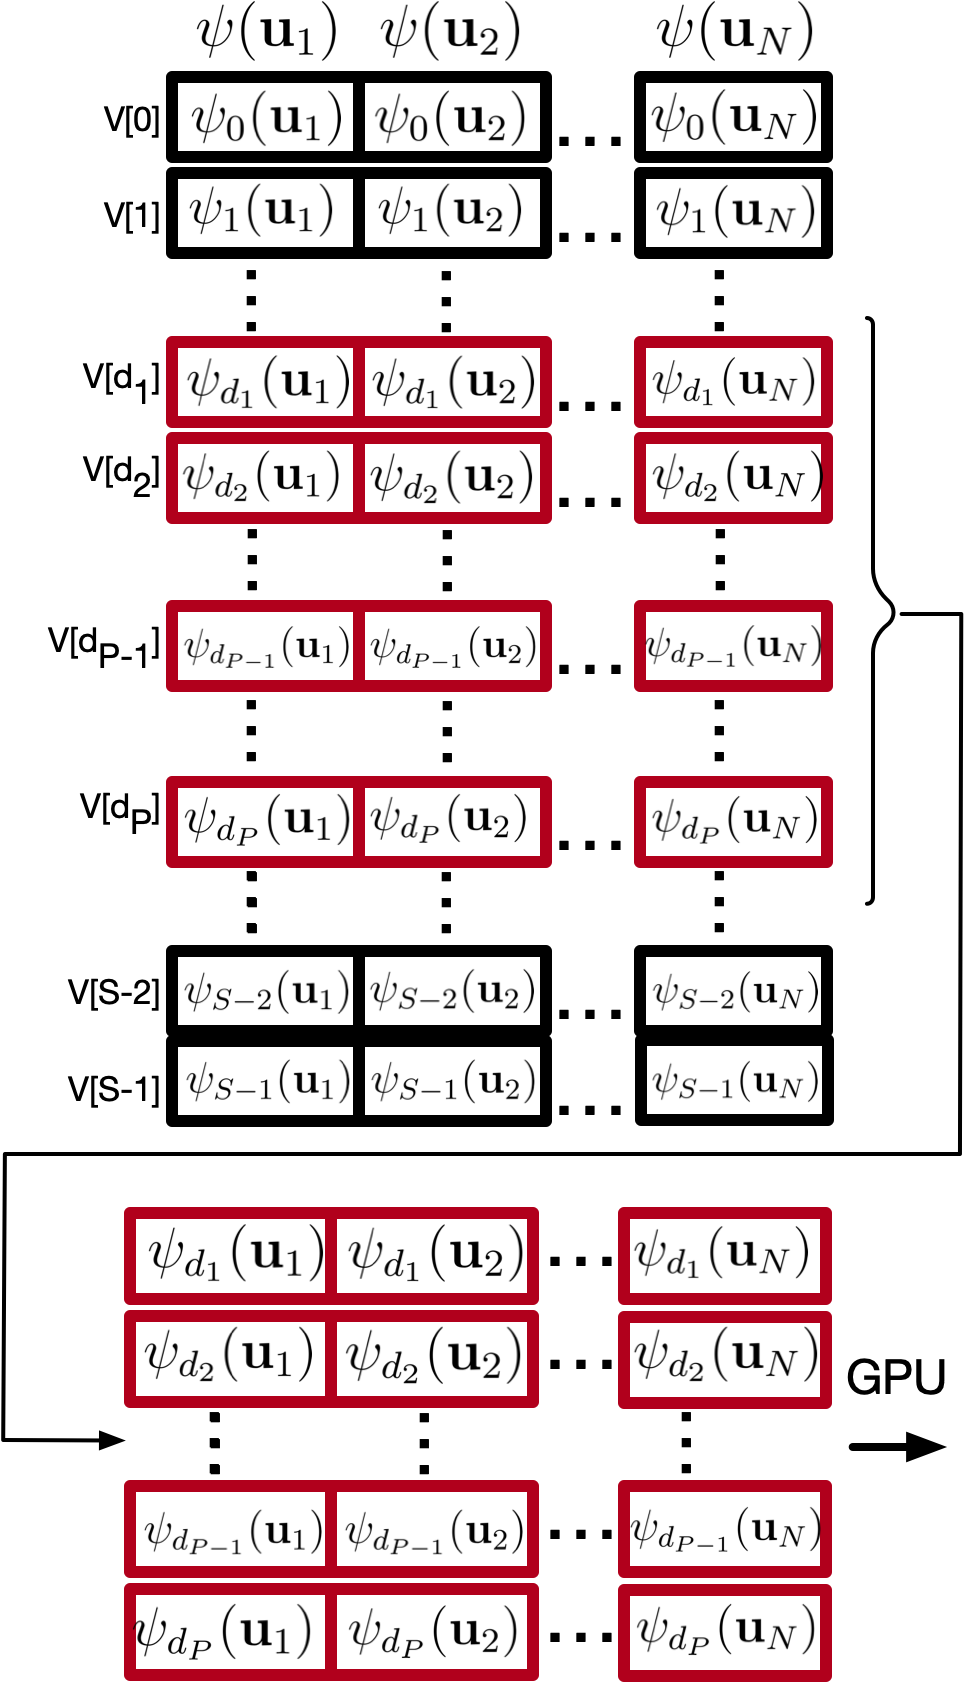
\includegraphics[width=0.89\linewidth, angle=0]{figs/rendering_scheme/organizacao2GPU_red1.png}
    \caption{Rendering scheme applied to a DWI visualization scheme. For each one of the $S$ DWI's samples, its respective ODF is pre-computed in $N$ samples in an hemisphere. The $P$ red-contoured ODFs are requested to be drawn, thus setting up the matrix $\bm{\Psi^{h}}$ and sent to the GPU. The ODF set can refer to a slice, for example}
    \label{fig::vmtk_precomputed2GPU}
\end{figure}


%\todo[inline]{To assess the fiber orientations locally?}

\subsection{Discussion}

One can make a comparison in an scheme where the per-glyph data traffic consists of vertices of triangles. Let us consider a N-size spherical mesh, where each point is a vertex of 6 triangles, which is characteristic of a tessellated icosahedron. The data traffic of our approach per glyph consists consists of N/2 floats plus one copy of translate coordinates, the customization of the glyphs are done per vertex in parallel in the GPU. The information on how to set the triangles are provided in the initialization process.

The polygon based approach proposed by Shattuck et al. \cite{shattuck2008} does not bring the discussion on the data structures sent to GPU in each drawing request and mention that they did not use GPU programming, furthermore, instance rendering was not available when the work was proposed. Certainly the glyph customization is done in CPU and the data traffic CPU-GPU consisted of a set of vertices extracted from the used spherical mesh with some redundancy, so the API can form triangles. It means that the amount of vertices data sent is higher than N, corresponding to more than 3*N floats for each glyph. Hence, the data traffic of our approach is less than 1/6 for the same spherical mesh.

%In our approach, that amount of data traffic goes to N/2 floats. Other polygon-based approaches, such as using sending vertices of the glyphs associated to an index buffer, makes the data traffic go to 3N floats plus the size of index buffer and, additionally, regarding translation coordinates, one can choose to send this data as an attribute per vertex and increase the data traffic by 3N floats and do on GPU's threads, or the operation can be done on CPU, which is less efficient than sending once per geometry.

%Shattuck et al. \cite{shattuck2008}  do not discuss the data structures sent to GPU in each drawing request and mention that they did not use GPU programming, so 

%the data traffic to setup a glyph is 6 times the same (x,y,z) coordinate of the modulated point, which translate to 18*N floats. If using triangle fan, where the same vertice can define two triangles, that amount goes to 9*N floats



Albeit we presented means to decrease CPU-GPU data traffic on this polygon-based approach, it is still much higher than the ray casting approaches. In their work, Peeters et al. \cite{peeters2009} mentions a data-traffic of 15 spherical harmonics coefficients per glyph and obtain smoother results than $3^{rd}$ and $4^{th}$ order tessellation of an icosahedron.


In contrast, these rendering strategies makes possible to increase the resolution of the sphere.

In comparison with Peeters et al. \cite{peeters2009}, our approach has much more data traffic, but the GPU shaders are much simpler an less intensive computationally than the approach suggested in their work.

%Falar da simplicidade é algo relevante?
%In our approach, the GPU shaders are much simpler than the raycasting approach since it only does a lookup on a texture and per-vertex linear transformations, while ray casting approaches bring are more computationally expensive.

%In MRI visualization tools, one may code a HARDI ODFs in two different ways: samples on a sphere and spherical harmonics coefficients. This rendering scheme is straightforward to be used when the data is coded in samples on a sphere, but approach to store HARDI data can be very memory demanding.





\section{Conclusions}
\label{sec::conclusions}

In this work, we presented a rendering scheme to render multiple ODFs at interactive rates. We used a polygons-based approach and suggested procedures to decrease the data traffic CPU-GPU in drawing requests.

We also suggested an optimization procedure to decrease the data computation and CPU-GPU data traffic by half on symmetrical ODFs.

The rendering scheme proved to be fast enough to render hundreds and thousands of objects using meshes that are fine sufficiently to make the surfaces appear smooth.

This scheme can be integrated with other DW-MRI and MRI visualization schemes and we exemplified an application. %It can be a useful tool to render each ODF's glyph on its respective area in the scene.

\subsection{Future works}

For future works, we will do the following investigations:
\begin{itemize}
\item provide in depth a performance comparison between the ray casting approach with the approach suggested in this work;
\item adapt the scheme by changing the data that customize the glyphs from ODF samples to spherical harmonics basis coefficients and compute its samples in GPU;
\item investigate strategies to change the spherical mesh as a function of the amount and size of glyphs to be rendered in a drawing request, giving the possibility of decreasing its number of vertices in situations where glyphs are small and/or in high number in the scene.
\end{itemize}







%\section{Page size}
%Permission to make digital or hard copies of all or part of this work for personal or classroom use is granted without fee provided that copies are not made or distributed for profit or commercial advantage and that copies bear this notice and the full citation on the first page. To copy otherwise, or republish, to post on servers or to redistribute to lists, requires prior specific permission and/or a fee. 

%All material on all pages should fit within a rectangle of 16 x 23.7 cm (6.3"x 9.33"), centered on the page horizontally, beginning 2.5 cm (1") from the top of the page and ending with 3,5 cm (1.4") from the bottom.  The right and left margins should be 2.5 cm (1"). The text should be in two 7.6 cm (3") columns with a 0.8 cm (0.3") gutter. 

%\section{Typeset text}
%\subsection*{Normal or Body Text}
%Please use a 10-point Times Roman font, or other Roman font with serifs, as close as possible in appearance to Times Roman in which these guidelines have been set. The goal is to have a 10-point text, as you see here. Please use sans-serif or non-proportional fonts only for special purposes, such as distinguishing source code text. If Times Roman is not available, try the font named Computer Modern Roman. On a Macintosh, use the font named Times.  Right margins should be justified, not ragged.

%\subsection*{Title and Authors}
%The title (Helvetica 18-point bold), authors' names (Helvetica 10-point) and affiliations (Helvetica 10 point) run across the full width of the page -- one column wide. We also recommend e-mail address (Helvetica 10 point). See the top of this page for three addresses. If only one address is needed, center all address text. For two addresses, use two centered tabs, and so on. For more than three authors, you may have to improvise.\footnote{If necessary, you may place some address information in a footnote, or in a named section at the end of your paper, but margins must remain empty.} 

%\subsection*{First Page Copyright Notice}
%Please include 3.8 cm (1.5") text box with the text shown at the bottom of the left column of the first page with the copyright notice.

%\subsection*{Others Pages}
%Others pages start at the top of the page (margin 2.5 cm) and continue in double-column format.  The two columns on the last even page should be as close to equal length as possible. 

%{\bfseries Total length of a paper is max. 8 pages.}

%Footnotes should be Times New Roman 9-point, and justified to the full width of the column.

%Please, use the standard Journal of WSCG format for references -- that is, a numbered list at the end of the article, ordered alphabetically by first author, and referenced by a name in brackets \cite{con00a}. See the examples of citations at the end of this document. Within this template file, use the style named references for the text of your citation.

%The references are also in 9 pt., but that section (see Section \ref{references}) is ragged right. References should be published materials accessible to the public. Internal technical reports may be cited only if they are easily accessible (i.e. you can give the address to obtain the report within your citation) and may be obtained by any reader. Proprietary information may not be cited. Private communications should be acknowledged, not referenced, e.g. "[Adam, personal communication]").

%\subsection*{Page Numbering, Headers and Footers}
%Do not include headers, footers or page numbers in your submission. These will be added when the publications are assembled.

%\begin{figure}[htb]
%    \centering
%    \rule{6cm}{3cm}
%    \caption{Insert caption to place caption below figure.}
%    \label{fig:box}
%\end{figure}

%\begin{table}[htb]
%	\centering
%	\begin{tabular}{|l|l|l|l|}
%	\hline
%	Graphics & Top & In-between & Bottom \\
%	\hline
%	Tables & End & Last & First \\
%	\hline
%	Figures & Good & Similar & Very well \\
%	\hline
%	\end{tabular}
%	\caption{Table captions should be placed below the table}
%\end{table}

%\section{Figures/Captions}
%Place Tables/Figures/Images in text as close to the reference as possible (see Fig.\ref{fig:box}). It may extend across both columns to a maximum width of 16 cm (6.3"). Captions should be Times New Roman 10-points.  They should be numbered (e.g., "Table 1" or "Figure 2"), please note that the word for Table and Figure are spelled out. Figure's and Table's captions should be centered beneath the image, picture or a table.

%\section{Sections}
%The heading of a section should be in Times New Roman 12-point bold in all-capitals flush left with an additional 6-points of white space above the section head.  Sections and subsequent sub- sections should be numbered and flush left. For a section head and a subsection head together (such as Section 3 and Subsection 3.1), use no additional space above the subsection head.

%\subsection{Subsections}
%The heading of subsections should be in Times New Roman 12-point bold with only the initial letters capitalized. (Note: For subsections and subsubsections, a word like the or a is not capitalized unless it is the first word of the header.)

%\subsubsection{Subsubsections}
%The heading for subsubsections should be in Times New Roman 11-point italic with initial letters capitalized and 6-points of white space above the subsubsection head.

%\section{Acknowledgments}
%Our thanks to ACM SIGCHI and SIGGRAPH for allowing us to modify templates they had developed.

%-------------------------------------------------------------------------
% example of algorithm typesetting
% to allow this, uncomment line 
% \RequirePackage[noend]{myalgorithm}
% in the wscg.sty file
% and download that package from Gabriel Zachmann's page http://zach.in.tu-clausthal.de/latex/
%
%
%\begin{algorithm}
%\hrule
%  \centering
%\begin{algorithmic}
%    \STMT $d_{l,r} = f_B(P_1), f_B(P_n)$
%    \WHILE{ $|d_l| > \epsilon $ and $|d_r| > \epsilon $ and $l<r$}
%        \STMT $d_x = f_B(P_x)$
%        \IF{ $d_x < 0$ }
%            \STMT $l, r = x, r$
%        \ELSE
%            \STMT $l, r = l, x$
%        \ENDIF
%    \ENDWHILE
%\end{algorithmic}
%\hrule
%\caption{Example of some pseudo-code}
%\label{fg:code}
%\end{algorithm}


%-------------------------------------------------------------------------

\printbibliography
%\begin{thebibliography}{99}
%\label{references}
%\label{references}
%\bibitem[And01a]{and01a} Anderson, R.E. Social %impacts of computing: Codes of professional %ethics. Social Science, pp.453-469, 2001.
%\bibitem[Con00a]{con00a} Conger., S., and Loch, %K.D. (eds.). Ethics and computer use. Com.of ACM %38, No.12, 2000.
%\bibitem[Con00b]{con00b} Mackay, W.E. Ethics, lies %and videotape, in Conf.proc. CHI'00, Denver CO, %ACM Press, pp.138-145, 2000.
%\bibitem[Jou01a]{jou01a} Journal of WSCG \& WSCG %templates: http://wscg.zcu.cz/jwscg/template.doc %(MSWord)
%http://wscg.zcu.cz/jwscg/template.pdf (PDF)
%\end{thebibliography}
%{\bfseries


%Last page should be fully used by text, figures etc. Do not leave empty space, please. 
%Do not lock the PDF -- additional text and info will be inserted, i.e. ISSN/ISBN etc. 
%}
\end{document}